\documentclass[12pt]{article}
\usepackage{amsmath}
\usepackage[margin=1in]{geometry}
\usepackage{setspace}
\usepackage{graphicx}
\usepackage [english]{babel}
\usepackage [autostyle, english = american]{csquotes}
\MakeOuterQuote{"}
\doublespacing

\graphicspath{{images/}{plots/}}

\author{Tyler Reisinger}
\title{Effect of Jupiter-sized Planet Interactions on Planetary Systems}
\date{}

\begin{document}

\begin{titlepage}
    \begin{center}
        \vspace*{1cm}
        
        \textbf{Effect of Strong Stellar Interactions on Planetary Systems and
            the Formation of Hot Jupiters}
        
        \vspace{1.5cm}
        
        \textbf{Tyler Reisinger}\\
        %\vspace{0.5cm}
        Under the guidance of Dr. Steve McMillan and Joseph Glaser
        
        \vfill
        
        Submitted in partial fulfillment of the requirements for the
        degree of Bachelor of Science in Physics
        
        \vspace{0.8cm}

        Department of Physics \\
        Drexel University \\
        Philadelphia, PA, United States\\
        26th of May, 2017 
    \end{center}
\end{titlepage}

\tableofcontents

\clearpage

\section{Abstract}

"Hot Jupiters" (HJs) are large planets that orbit very close to their host star. 
They appear to be somewhat commonly occurring in the universe, with approximately 1\% 
of sun-like solar systems predicted to contain one (A. Brucalassi et al. 2016). 
However, the mechanism that causes these planets to have such extreme orbital parameters
is not fully understood. 
We aim to explore the role that star-planet and planet-planet gravitational interactions 
within a star cluster may have in producing Hot 
Jupiters. By using computational simulations of "typical" star clusters,
we will attempt to probe what happens over vast periods of time
in star clusters similar to those found within the observable universe.
We will run detailed simulations of close stellar encounters within these clusters
and observe the resulting state of the systems after the stars have separated. Many
of these system may then be stored and computationally analyzed. 
As a result of these simulations, 
we hope to observe the formation of Hot Jupiter-like orbits that
match observational data as well as determine how common an occurrence.
Additionally, we will observe what other damage might 
persist within the planetary orbits of the system that can be used as 
observational evidence for this formation scenario. Finally, we will
produce a collection of code which may be used in the future to perform similar
experiments.

\clearpage

\section{Introduction}

In the study of exoplanets, one interesting class of planets are the so-called "Hot Jupiters" -- planets with near-Jupiter mass that have a 
very small radius orbit around their host star. 
Hot Jupiters are interesting as their orbits approach very close to the host star,
despite the fact that most Jupiter-mass planets are considered to form much farther
out -- in the accretion disk of the forming planetary system. If we look at our own
solar system, we see that Jupiter orbits at around 5.2 Astronomical Units (AU) from the
sun, where one AU is approximately the average orbital distance of the Earth. Indeed,
we see a very large gap between the orbits of the inner, small and rocky planets, and
the outer gas planets, of which Jupiter is the nearest. Jupiter is not an anomaly of
the universe, but rather most gas giants are seen in a similar orbit. 

The Hot Jupiters seen in the universe, however, have orbital 
radii of only fractions of an AU, potentially 
approaching their star closer than even Mercury in our own solar system.
This is well beyond the accretion disk, and there must, then, be a difference between
the "average" Jupiter planet such as what is found in our solar system, and these
extreme Hot Jupiters.

The mode of formation for these Hot Jupiters is not fully understood.
Despite this, and their rather exotic orbits, 
they appear to be somewhat common within the universe as observations and previous models place the occurrence of Hot Jupiters at around 1\% of all solar systems (A. Brucalassi et al. 2016).  

A likely aspect of the formation of these Hot Jupiters is that they are not formed in place, but rather form much like normal gas giant planets 
in a gas accretion disk beyond the ice line. They then migrate to their final close orbit sometime later after their formation. 
In order for the Hot Jupiter to move into a close orbit after it is formed, some sort of interaction must occur to change the orbital parameters. 
Disk migration theory postulates that the accretion of gases and 
solids during the planet's formation process also slowly alters the orbital 
parameters of the planet,
pushing the planet inward towards the star.
This is thus a potential mechanism for the creation of these Hot Jupiters, but is not the end of the story.

Within a star cluster, there are times when two stellar systems approach very close
to one another. Depending on the closeness of the approach, the effects of such
an interaction may very. A few hundred AU encounter will likely disturb the trajectory
of the two stars in the short term, and most of the encounters will end here. However,
if the two stars become close enough that the approaching star's gravitational attraction
overtakes that of the host star, the planets around each star may have their orbits
highly disturbed. In this case, more distantly orbiting planets, such as the gas giants
have a greater chance to disturbed than the inner planets like Earth.

This gravitational "push" could also have many effects on the unlucky planets caught in the
middle. One likely outcome is that the orbit is made more eccentric but otherwise
mostly unchanged. Additionally, the planet could be ejected from the planetary system,
or be caught by the approaching star. A third possibility is that a Jupiter-like planet
from the outer solar system is thrown into an orbit that approaches much closer to the
star. In such a case, the orbit right after the interaction should have a highly
eccentric orbit, even if it passes close to the host star. Orbital decay over long
timescales would be required to "circularize" such orbits into something more regular.

Additionally, the inward movement of the larger gas planet could affect other
inner planets of the solar system during its transit. This would similarly 
cause the inner planet orbits to become more eccentric and could move
these planets closer or farther from the star depending on the details of the
interaction, or even eject them out of the system. Should this occur,
then another "pair" planet could be formed in the same system. This would leave
a second long-term impact on the system, if present, may provide observational
evidence for this theory.

Such an interaction also holds importance for the fate of the affected Earth-like planets.
A planet formerly in the habitable zone of a star could be knocked into a far less
forgiving orbit, leading to likely fatal effects on life. Additionally, a
large planet in an eccentric orbit that passes within the inner planetary orbits,
even if it does not perturb these planets right away, might lead to later chance
encounters between the planets that lead to orbital changes.

We will focus on the star cluster interactions. Using computer simulation,
we may attempt to probe the gravitational dynamics of these star system 
interactions in time scales much more relevant to human life. We will simulate
a large number of these interactions, building up a database of information about
the initial and final states of the systems. From this data, we may perform large
scale analyses, finding potential Hot Jupiter formation events, as well as other
significant perturbations to the planetary orbits.

By having a large database of encounter information, we may also looks for commonalities
and frequencies of the destructive events encountered. 

%TODO: Finish this

\section{Methods}

    Our approach was entirely computational in nature. We developed a collection of tools
    and utilities utilizing the popular Python programming language and making use
    of the AMUSE (Astrophysical Multipurpose Software Environment) library. 
    %TODO: Verify how to write the name

    AMUSE provides the underlying gravitational simulation methods, with many different
    integrators and utilities for different needs. With AMUSE, we were able to 
    setup our problem and tell AMUSE to return to our code for encounter events and
    let AMUSE handle the rest. Additionally, AMUSE provides these features in high
    performance C++ and Fortran kernels, allowing us to focus on functionality without
    worry about the gravitational simulation details.

    N-body gravitational simulations with high accuracy and over long time scales requires
    a significant amount of computationally expensive numerical integration of the 
    forces involved in the experiment. In order to exploit the parallel nature of 
    the simulations, our code was run mostly on the Draco computer 
    cluster at Drexel University. This cluster provides 24 connected nodes, each containing
    a significant number of CPU cores as well as a few GPUs. Utilizing this cluster,
    we were able to run many simulations in parallel.

    \subsection{Overview}

    The code has three logical phases. The first phase is to run simulations of typical
    star clusters and to record all "close encounters" between stars in the cluster.
    At this stage, there are no planets around the stars, but rather we will use the
    parameters of the close encounters to run more detailed simulations in isolation
    later.

    The second phase is running those detailed simulations. A pair of interacting stars
    is placed into the simulation with the same dynamic parameters as in the cluster,
    and planets are added around each. A much shorter gravitational simulation is then
    run, allowing the systems to approach, interact and later separate. The final
    state of the two systems are recorded for the next phase.

    The final phase is to analyze the data generated from the previous simulations.
    Many simulations are run in order to develop a diverse profile of interactions.
    At this phase, we look for interesting encounters, what events are most common
    and the approximate frequency of certain outcomes. From here, the results could
    be used to verify the validity of the simulations with observation and to make
    predictions about these events in the universe.

    %TODO: Describe binary orbital parameters.

    \subsection{N-Body Simulation}

    The N-Body simulation code was the first part the code to be completed. In the
    universe, the dynamics of the star cluster and the dynamics of the
    interactions of planets around the containing stars are, of course, happening
    simultaneously. However, the dynamics of stars in a cluster are changing much
    more slowly than those of the planets because of the much larger distances
    involved. While a planet can fully rotate about a star in less than a year,
    only a handful of stars pass close to one another in a megayears. Accurately
    simulating planets around stars within a star cluster would require
    far more computation time, and most of this would be wasted simulating
    planets normally orbiting their host star far away from any other stars.

    The gravitational effects of an external star on a planet's orbit only
    causes noticeable orbital effects if the star comes very close (within 10-20AU)
    of the planet itself. This means that a Jupiter-like planet with an orbit around
    5 AU would only potentially be perturbed by a star that comes within 
    approximately 30 AU of the host star. Indeed, experimentally, we observe that
    encounters more distant than this leave almost no visible impact on the
    interacting systems. 

    Since we only care about the fate of planets during one of these 
    rare close encounters,
    the clusters created for these simulations are composed entirely of planet-less stars.
    Each gravitational simulation of a cluster is performed for between 50 
    and a few hundred megayears. During the simulation, any time two stars
    come close enough to strongly interact, the simulation is briefly halted so that
    the dynamical and orbital parameters can be recorded. The simulation is then
    resumed and this process repeats. At the end, a file is generated with
    all close encounters observed during the simulation, as well as the initial
    cluster bodies and information about the simulation itself.

    A "close encounter" as defined by this part of the code is when two stars
    come close enough to have a strong encounter between them. AMUSE decides
    this distance itself and notifies the simulation when this occurs. For planetary
    effects, we are generally uninterested in the majority of these encounters, however
    we choose to record all of these encounters for later filtering based on the
    planets being studied. For example, if in the future we were to add Neptune-like
    planets into the planetary systems, orbiting around 30 AU from the sun, we would
    be interested in more distant encounters than when using a Jupiter as the most
    outer planet.

    The clusters generated for the simulation are uniquely created each time at the
    beginning of the simulation using a pseudo-random number generator. 
    The star properties are sampled from a
    King Model with a fixed $W_0=3.0$. %TODO: Mass Stuff
    All stars added to the cluster are given a fixed mass $M=M_{sun}$ and do not
    include any binary star systems. The number
    of stars in the cluster were varied between 1000 and 10000. 

    \begin{figure}
        \centering
        \caption{Two clustered generated and used for simulation superimposed.}
        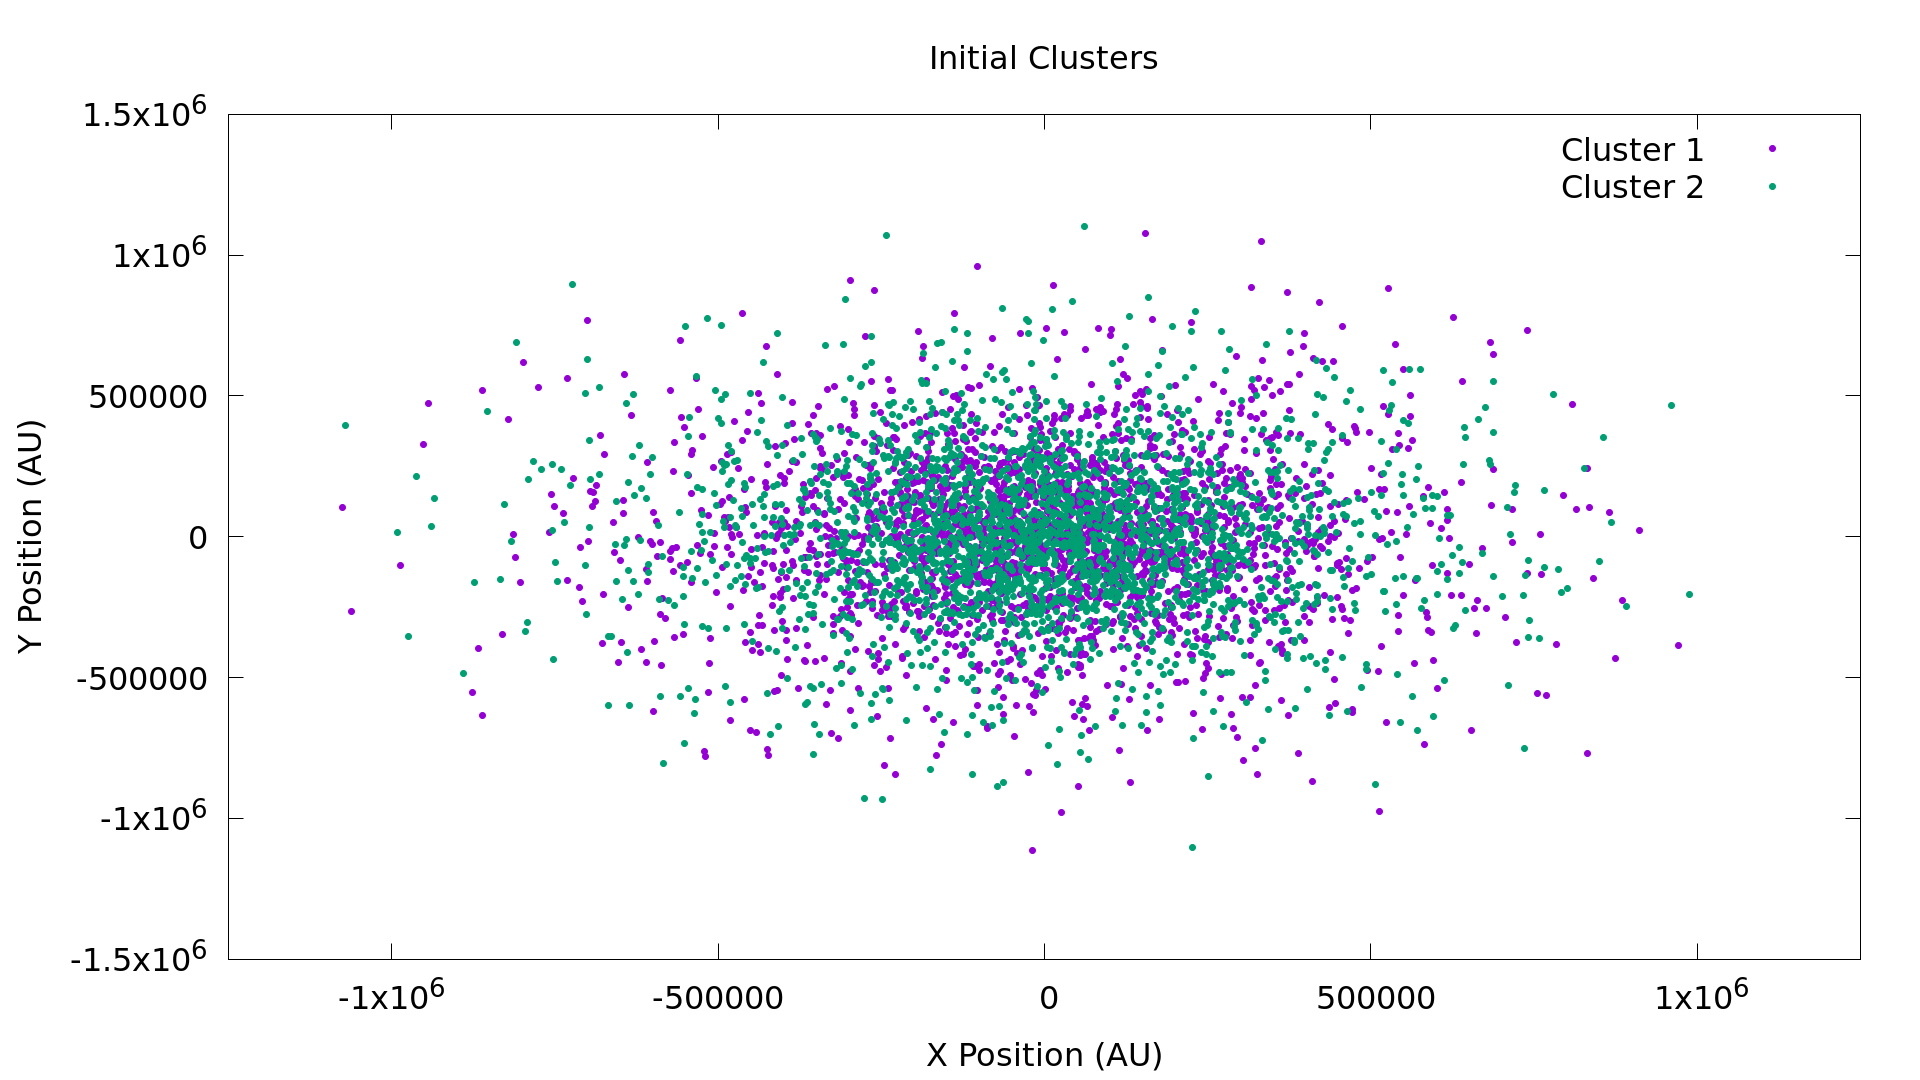
\includegraphics[width=4.0in]{cluster_superimposed.png}
    \end{figure}

    Each 100 megayears of simulation time for one of these clusters yields a
    few hundred encounters on average. The close encounters given to our by 
    AMUSE are based on the distance of the two stars at the present simulation time.
    Since the most distant encounters where the two stars get little closer to one
    another than this are mostly uninteresting to us, we also need to understand
    the approximate distance of closest approach for these stars. Fortunately, treating
    the interacting stars as a binary system allows us to compute the orbital parameters
    of the interaction. 

    %TODO: Blah

    %TODO: Add closest approach spectrum

    %TODO: Encounter distance vs distance of closest approach
    

    \subsection{Monte Carlo}

    From the N-Body simulation, a list of star encounters for any number of 
    clusters may be generated. The next step is to read these encounters and
    simulate just the two stars involved for each in isolated from the 
    environment. In addition, planets are added around both stars in the
    encounter before they are added to the simulation. The initial positions,
    velocities and physical parameters of the stars are identical to what they
    were at the moment AMUSE identified them as interacting. 

    Once the stars are setup with their planets, their gravitational dynamics
    are simulated. As the stars have just started interacting, the stars should
    move toward each other, reach a point of closest approach and then separate again
    in hyperbolic orbits.

    In the next phase of the experiment, we define a "close encounter" to be
    one where the closest approach between two stars is 30 AU or less and discard
    all other encounters from the dataset. 

    %Two figures of interacting systems

    \subsection{Analysis}

    %Some analysis pictures


\section{Results}

    %Data management

    %Runtime considerations

    %Future?

\section{Conclusion}

We explored a potential formation scenario for the formation of Hot Jupiter
planets. These planets have been observed in the universe with some frequency,
but their exact method of formation remains debated. 
We theorize that strong interactions between two planetary systems in a star
cluster could perturb the orbit of a normal gas giant to approach very close to
its host star. 

Our simulations show that this is indeed a possibility, and that very close
interactions on the order of a few AU can frequently throw Jupiter-mass planets into
highly eccentric orbits with very close approaches to the host star. 
This may then also drastically impact the orbits of other planets
in the system. This provides support for the idea that a Hot Jupiter may very
often have another pair planet that was thrown into an extreme orbit by the same
process that affected the Jupiter's orbit. Thus,
observation of these pair planets may provide reason to search for a Hot Jupiter
nearer the star.
Further long-term simulation would be needed to see if the highly eccentric Jupiter
orbit could decay into a more circular orbit similar to many observed Hot Jupiters.

\clearpage

\begin{thebibliography}{9}

\bibitem{James B. Pollack et al. 1996}
James B. Pollack, Olenka Hubickyj, Peter Bodenheimer, Jack J. Lissauer, Morris Podolak, Yuval Greenzweig, Formation of the Giant Planets by Concurrent Accretion of Solids and Gas, Icarus, Volume 124, Issue 1, 1996, Pages 62-85, ISSN 0019-1035, http://dx.doi.org/10.1006/icar.1996.0190.
(http://www.sciencedirect.com/science/article/pii/S0019103596901906)

\bibitem{A. Brucalassi, 2016}
A.  Brucalassi, L.  Pasquini, R.  Saglia, M. T.  Ruiz, P.  Bonifacio, I.  Leão, B. L.  Canto Martins, J. R.  de Medeiros, L. R.  Bedin, K.  Biazzo, C.  Melo, C.  Lovis, S.  Randich,
Search for giant planets in M67 - III. Excess of hot Jupiters in dense open clusters
A\&A 592 L1 (2016)
DOI: 10.1051/0004-6361/201527561

\bibitem{Foreman-Mackey et al. 2016}
Foreman-Mackey, D., Morton, T.~D., Hogg, D.~W., Agol, E., \& Sch{\"o}lkopf, B.\ 2016, arXiv:1607.08237 

\bibitem{Shara et al. 2014} Shara, M.~M., Hurley, J.~R., \& Mardling, R.~A.\ 2014, arXiv:1411.7061 

\end{thebibliography}

\end{document}
